%% PREAMBLE
\documentclass[xcolor=dvipsnames,10pt]{beamer}
\setbeamercovered{transparent} % dim inactive elements

% general theme
\usetheme{Madrid}

% inner theme
\useinnertheme{circles}

% color scheme
\definecolor{UBCblue}{rgb}{0.04706, 0.13725, 0.26667}
\definecolor{UBCgrey}{rgb}{0.3686, 0.5255, 0.6235}
\setbeamercolor{palette primary}{bg=UBCblue,fg=white}
\setbeamercolor{palette secondary}{bg=UBCblue,fg=white}
\setbeamercolor{palette tertiary}{bg=UBCblue,fg=white}
\setbeamercolor{palette quaternary}{bg=UBCblue,fg=white}
\setbeamercolor{structure}{fg=UBCblue}
\setbeamercolor{section in toc}{fg=UBCblue}
\setbeamercolor{subsection in head/foot}{bg=UBCgrey,fg=white}

% turn off ugly footer
\setbeamertemplate{footline}[frame number]{}
\setbeamertemplate{navigation symbols}{}

% fonts
\usefonttheme{professionalfonts} % using non standard fonts for beamer
\usefonttheme{serif} % default family is serif
\usepackage{fontspec}
\setmainfont{Liberation Serif}

% hyphenation for letterspacing and text decoration
\usepackage{soul}

% references
\usepackage[backend=biber,style=authoryear-icomp]{biblatex}
\addbibresource{bibl.bib}
\makeatletter
\renewrobustcmd{\blx@mkbibfootnote}[2]{%  deal with columns
  \iftoggle{blx@footnote}
    {\blx@warning{Nested notes}%
     \addspace\mkbibparens{#2}}
    {\unspace
     \ifnum\blx@notetype=\tw@
       \expandafter\@firstoftwo
     \else
       \expandafter\@secondoftwo
     \fi
       {\csuse{blx@theendnote#1}{\protecting{\blxmkbibnote{end}{#2}}}}
       {\csuse{footnote#1}[frame]{\protecting{\blxmkbibnote{foot}{#2}}}}}}
\makeatother

% SI units in text and stuff related to math, tables, etc.
\usepackage[detect-all]{siunitx}
\sisetup{per-mode=symbol,range-phrase=--,range-units=single}
\usepackage{amsmath}
\usepackage{booktabs}

% figures
\usepackage{tikz}
\usetikzlibrary{calc, positioning, shapes, backgrounds, fit, arrows}
\usepackage{pgf-spectra}
\usepackage{contour}
\usepackage{adjustbox}
\usepackage{wrapfig}
\def\checkmark{\tikz\fill[scale=0.4](0,.35) -- (.25,0) -- (1,.7) -- (.25,.15) -- cycle;}
\usepackage{caption}
\usepackage{subcaption}

% the title slide with my information
\setbeamertemplate{title page}[default][wd=\textwidth,rounded=false]
\title{Advanced technique for assessment of spatially averaged dosimetric quantities on non-planar surfaces}
\subtitle{Proposal of the dissertation topic}
\author[Ante Kapetanović]{Ante Kapetanović}
\institute{Faculty of Electrical Engineering, Mechanical Engineering and Naval Architecture (FESB)}
\date{\today}
\titlegraphic{\includegraphics[height=1.25cm]{figures/logo/unist.png}}


%% DOCUMENT
\begin{document}

% generate the title slide
\begin{frame}[plain]
    \maketitle
    \begin{center}
        \scriptsize{%
            Jury Members\par
            President: prof Zoran Blažević, PhD\par\medskip
            \begin{table}
                \centering
                \begin{tabular}{llll}
                Examiners: & prof Zvonimir Šipuš, PhD & Supervisor: & prof Dragan Poljak, PhD \\
                 & assoc prof Vicko Dorić, PhD &  &  \\
                 & assoc prof Mario Cvetković, PhD &  & 
                \end{tabular}
            \end{table}
        }%
    \end{center}
\end{frame}

% the main table of contents
\begin{frame}{Table of contents}    
    \setbeamertemplate{section in toc}[sections numbered]
        \tableofcontents
\end{frame}

% a table of contents that appear before new section
\AtBeginSection[]{
    \begin{frame}{Table of contents}
        \setbeamertemplate{section in toc}[sections numbered]
        \tableofcontents[currentsection,hideallsubsections]
    \end{frame}
}

% introductory section
\section[Introduction]{Introduction}

\subsection{Problem and object of scientific research}
\begin{frame}{Problem and object of scientific research}
    \begin{itemize}
        \item the rise of data-intensive wireless devices $\rightarrow$ expansion of the utilized radio frequency (RF) spectrum into millimeter waves (MMW)\footcite{Rappaport2013Millimeter}
        \item global roll-out of the fifth-generation (5G) standard for broadband cellular networks $\rightarrow$ improved communication performance by increasing channel capacity and reducing network latency through\footcite{Andrews2014What}:
        \begin{itemize}
            \item carrier aggregation
            \item multiple-input multiple-output (MIMO) technology
            \item beam-forming (or spatial filtering)
            \item frequency range (FR) 1 (\SIrange{0.45}{6}{\GHz}), FR 2 (\SIrange{24.25}{52.6}{\GHz})
        \end{itemize}
        \item a growing public concern about adverse health effects from exposure to RF electromagnetic (EM) radiation\footcite{Wu2015Safe}
        \item to ensure absolute safety, various international bodies prescribe \emph{exposure limits} derived upon relevant scientific literature
    \end{itemize}
\end{frame}

\begin{frame}{But what is EM radiation?}
    \input{figures/em_spectrum.tex}
\end{frame}

\begin{frame}{Non-ionizing EM radiation effects
on biological tissue}
    \begin{itemize}
        \item a \emph{biological effect} $\rightarrow$ any change (physical, chemical, or mechanical) induced in tissue\footcite{ICNIRP2020Principles}
        \item feedback repair mechanism $\rightarrow$ preservation of homeostasis within \emph{threshold limits}
        \item limits exceeded $\rightarrow$ \emph{adverse health effect}\footcite{WHO2022Health}
        \item interaction effects $\rightarrow$ frequency-dependent
        \begin{tabular}{p{2.7cm}p{8cm}}
            static fields & induced fields and currents within tissue\\
            \SIrange{0}{0.1}{\MHz} & stimulation of excitable cells\\
            \SIrange{0.1}{10}{\MHz} & stimulation of excitable cells, tissue heating\\
            above \SI{10}{\MHz} & tissue heating exclusively
        \end{tabular}
        \item increase in frequency $\rightarrow$ absorbed power is dissipated predominately across the surface of the exposed tissue\footcite{Ziskin2018Tissue}
        \end{itemize}
\end{frame}

\begin{frame}{Exposure limits to artificial EM fields}
    \begin{itemize}
        \item prescribed by internationally recognized guidelines\footcite{ICNIRP2020Guidelines} and standards\footcite{IEEE2019Standard}
        \item protection against adverse health effects by respecting the frequency- and exposure scenario-dependent limits
        \item reduction factors applied in a conservative manner (inter-individual variability, uncertainties related to exposure setup or environment, etc.)
        \item threshold values $\rightarrow$ \emph{basic restrictions} or (BR) $\rightarrow$ \emph{reference levels} (RL)
        \begin{itemize}
            \item whole-body or localized exposure
            \item brief or steady-state exposure
        \end{itemize}
        \item the \emph{specific absorption rate} (SAR) used as BR for the steady-state core (whole-body average) and localized (10-g average) temperature rise from \SI{100}{\kHz} to \SI{300}{\GHz}
        \item the \emph{incident power density} in free space used as RL to provide practical means of demonstrating compliance
    \end{itemize}
\end{frame}

\begin{frame}{Exposure assessment and dosimetry in era of 5G}
    \begin{columns}[c]
        \begin{column}{0.5\textwidth}
             \begin{itemize}
                \item<1> at \SI{6}{\GHz}, \SI{90}{\percent} of the power is absorbed within the uppermost layer of the exposed tissue
                \item<2> BR set in terms of the area-averaged \emph{absorbed power density} (APD)
                \item<3> line integral of SAR depth-wise into the tissue $\rightarrow$ \emph{transmitted power density} (TPD)
                \item<4> area-averaged TPD $\equiv$ area-averaged APD $\rightarrow$ consistency and continuity with volume-averaged SAR
            \end{itemize}
        \end{column} 
        \begin{column}{0.5\textwidth}
            \begin{onlyenv}<1>
                \begin{center}
                \begin{figure}
                    \includegraphics[width=\textwidth]{figures/penetration_depth.pdf}
                    \caption{Penetration depth and transmission coefficient as a function of frequency.}
                \end{figure}
                \end{center}
            \end{onlyenv}
            \begin{onlyenv}<2>
                \begin{center}
                \begin{figure}
                    \includegraphics[width=0.7\textwidth]{figures/averaging_surface.a.pdf}
                    \caption{Averaging area on the exposed tissue surface from 3-D point of view.}
                \end{figure}
                \end{center}
            \end{onlyenv}
            \begin{onlyenv}<3>
                \begin{center}
                \begin{figure}
                    \includegraphics[width=0.7\textwidth]{figures/averaging_surface.b.pdf}
                    \caption{Averaging area on the exposed tissue surface from the lateral point of view.}
                \end{figure}
                \end{center}
            \end{onlyenv}
            \begin{onlyenv}<4>
                \begin{center}
                \begin{figure}
                    \includegraphics[width=0.7\textwidth]{figures/exposed_tissue_volume.pdf}
                    \caption{A cube of tissue for the volumetric averaging of SAR during localized steady-state exposure.}
                \end{figure}
                \end{center}
            \end{onlyenv}
        \end{column}
    \end{columns} 
\end{frame}

\begin{frame}{Mathematical definition of APD}
    \begin{columns}[c]
        \begin{column}{0.4\textwidth}
            \begin{itemize}
                \item recent major revisions of IEEE/ICES standard (in 2019) and ICNIRP guidelines (in 2020) have identified two definitions of the spatially averaged APD:
                \begin{enumerate}
                    \item<1> area-averaged power density flux
                    \item<2> area-averaged TPD
                \end{enumerate}
            \end{itemize}
        \end{column} 
        \begin{column}{0.6\textwidth}
            \begin{onlyenv}<1>
                \begin{equation*}
                    \centering
                        sPD_\text{ab, 1} = \frac{1}{2A} \iint_{A} \Re \big[\boldsymbol{E} \times \boldsymbol{H}^* \big] \; \boldsymbol{\hat n} \; \mathrm{d}A
                \end{equation*}
                \begin{itemize}
                    \item $\boldsymbol{E}$, $\boldsymbol{H}$ -- peak values of the complex phasor electric and magnetic field on the surface
                    \item $A$ -- frequency-dependent averaging area
                    \item $\boldsymbol{\hat n}$ -- unit normal vector on $A$
                    \item $\mathrm{d}A$ -- integral area element
                \end{itemize}
            \end{onlyenv}
            \begin{onlyenv}<2>
                \begin{equation*}
                    \centering
                    sPD_\text{ab, 2} = \frac{1}{A} \iint_{A} \int_{z} \rho \; \text{SAR} \; \mathrm{d}z \; \mathrm{d}A
                \end{equation*}
                where
                \begin{equation*}
                    \centering
                    \text{SAR} = \frac{\sigma \big| \boldsymbol{E} \big|^2}{2\rho}
                \end{equation*}
                \begin{itemize}
                    \item $\boldsymbol{E}$ -- peak value of the complex phasor electric field within tissue
                    \item $\sigma$ -- conductivity of tissue
                    \item $\rho$ -- tissue density 
                \end{itemize}
            \end{onlyenv}
        \end{column}
    \end{columns}
\end{frame}

\begin{frame}{Mathematical definition of IPD}
    \begin{itemize}
        \item IPD is defined as the modulus of the time-averaged Poynting vector assuming free space conditions
        \begin{equation*}
            \centering
            S_\text{inc} = |\boldsymbol{E} \times \boldsymbol{H}^* \big|
        \end{equation*}
        \item multiple definitions of the spatially averaged IPD have been proposed and dicussed\footcite{IEEE2021Guide} with two standing out in particular:
        \begin{enumerate}
            \item the normal component of the time-averaged Poynting vector
            \begin{equation*}
                \centering
                sPD_\text{inc, n} = \frac{1}{2A} \iint_{A} \Re \big[\boldsymbol{E} \times \boldsymbol{H}^* \big] \; \boldsymbol{\hat n} \; \mathrm{d}A
            \end{equation*}
            \item the magnitude of the time-averaged Poynting vector
            \begin{equation*}
                \centering
                sPD_\text{inc, tot} = \frac{1}{2A} \iint_{A} \big| \boldsymbol{E} \times \boldsymbol{H}^* \big|\; \mathrm{d}A
            \end{equation*}
        \end{enumerate}
    \end{itemize}
\end{frame}

\begin{frame}{Practical considerations for the averaging area}
    \begin{itemize}
        \item \SIrange{2}{6}{\GHz} $\rightarrow$ peak value of the power density
        \item $\geq$ \SI{6}{\GHz} $\rightarrow$ averaging on \SI{4}{\cm\squared} square evaluation plane\footcite{Hashimoto2017On,Funahashi2018Averaging}
        \item $\geq$ \SI{30}{\GHz} $\rightarrow$ averaging on \SI{1}{\cm\squared} square evaluation plane in addition to account for narrow beam formation\footcite{Foster2016Thermal}
        \item the power density spatially averaged on \SI{1}{\cm\squared} area should not exceed twice the value of the \SI{4}{\cm\squared} area \footcite{ICNIRP2020Guidelines}
    \end{itemize}
\end{frame}

\subsection[Related work]{Related work}
\begin{frame}{Tissue models and averaging area}
    \begin{columns}[c]
        \begin{column}{0.5\textwidth}
            \begin{itemize}
                \item above \SI{6}{\GHz}, planar tissue-equivalent single- or three/four-layer models commonly utilized\footcite{Zhadobov2011Millimeter}:
                    \begin{itemize}
                        \item stratum corneum
                        \item viable epidermis and dermis
                        \item hypodermis
                        \item muscle
                    \end{itemize}
                \item dielectric properties $\leftarrow$ four-term Cole-Cole model\footcite{Gabriel1996Compilation}
                \item the construction of the averaging area on a planar evaluation surface -- IEC/IEEE 63195-2:2022 international standard
            \end{itemize}
        \end{column}
        \begin{column}{0.5\textwidth}
            \begin{center}
            \begin{figure}
                \includegraphics[width=0.75\textwidth]{figures/Li2021Figure2_adjusted.pdf}
                \caption{Skin models with different tissue compositions and the exposure condition. Taken from the recent international inter-comparison study by Li et al. 2021.}
            \end{figure}
            \end{center}
        \end{column}
    \end{columns}
\end{frame}

\begin{frame}{Current state of the research: a short synthesis}
    \begin{itemize}
        \item from SAR to IPD, transition frequency of \SI{6}{\GHz}\footcite{Anderson2010SAR,McIntosh2010SAR}
        \item harmonization of the area of an evaluation surface between guidelines and standards\footcite{Colombi2015,Thors2016Exposure,Xu2017Understanding}
        \item \SIlist{4;1}{\cm\squared} square averaging area on a planar evaluation surface\footcite{Hashimoto2017On,Funahashi2018Averaging,Foster2016Thermal,Foster2017Thermal}
        \item the first mention of the spatially averaged TPD as a potential BR above \SI{6}{\GHz}\footcite{Funahashi2018Area-Averaged}
        \item validity of the IPD\footcite{Sasaki2017Monte,Li2019Relationship,He2018RF,Diao2021Effect,Carrasco2019Exposure,Miura2021Power,Nakae2020Skin,Morimoto2022Assessment} -- correlation with the resultant surface temperature rise under various exposure conditions and different skin and antenna models is satisfactory (Pearson coefficient $>$ 0.7, $p < 0.05$)\footcite{DeSantis2022On}
        \item validity of the APD\footcite{Li2021Quantitative,Taguchi2022Computation,Li2023Calculated} -- by using the heating factor\footcite{Foster2018Modeling}
    \end{itemize}
\end{frame}

\begin{frame}{Beyond the state of the art}
    \begin{columns}[c]
        \begin{column}{0.5\textwidth}
            \begin{itemize}
                \item non-planar body parts, e.g., fingers\footcite{Li2012Mechanisms}, ears\footcite{Sacco2022Exposure}, with the curvature radius $\sim$ wavelength of the incident EM field $\rightarrow$ underestimation of the area-averaged quantities
                \item non-planar tissue models currently discussed within IEEE ICES TC95 SC6 WG7
                \begin{itemize}
                    \item canonical shapes, e.g., sphere or cylinder\footcite{Diao2020Assessment,Kapetanovic2022AssessmentTEMC}
                    \item anatomical tissue models\footcite{Kapetanovic2022AssessmentJERM}
                \end{itemize}
            \end{itemize}
        \end{column}
        \begin{column}{0.5\textwidth}
            \begin{center}
            \begin{figure}
                \includegraphics[width=0.95\textwidth]{figures/Diao2020Figure2_adjusted.pdf}
                \caption{Reference averaging volumes/areas for different APD computation schemes. Taken from the study by Diao, Rashed and Hirata 2020.}
            \end{figure}
            \end{center}
        \end{column}
    \end{columns}
\end{frame}

\subsection{Motivation, purpose and objectives of the research}
\begin{frame}{Motivation, purpose and objectives of the research}
    \begin{itemize}
        \item to quantitatively and qualitatively \emph{investigate the influence of tissue surface morphology} on the values of extracted APD and IPD values above 6 GHz
        \item to develop an \emph{accurate numerical integrator} for spatial averaging of power flow regardless of the numerical/analytical technique used in EM field calculations
        \item to develop a \emph{computationally efficient automatic detection of the worst case scenario} -- the ``hot-spot'' region -- on the exposed surface of arbitrarily shaped tissue
    \end{itemize}
\end{frame}

\subsection{Hypothesis}
\begin{frame}{Hypothesis}
    \begin{enumerate}
        \item<only@1> traditional flat surfaces for the spatial averaging of the power density is inadequate for RF EM fields with wavelengths comparable to the approximate curvature radius of the non-planar body parts exposed
        \item<only@2> anatomical models with irregularities and asymmetries characterized by intricate convex-concave tissue structures on the surface require the high fidelity numerical estimation of unit vectors normal on the surface
        \item<only@3> heterogeneous EM absorption in the near field require evaluating the spatially averaged power density over the entire exposed surface
    \end{enumerate}
    \begin{block}{Assumption 1}<1->
        cylindrical or spherical models are better suited for practical compliance assessment for exposure of common non-planar body parts, e.g., fingers, outer ear, head
    \end{block}
    \begin{block}{Assumption 2}<2->
        the distribution of normal vectors significantly affects the absorption of the incident EM field
    \end{block}
    \begin{block}{Assumption 3}<3->
        hybridization of machine learning and traditional numerical methods can effectively detect worst-case exposure scenario
    \end{block}
\end{frame}


% materials and methods section
\section[Materials and methods]{Materials and methods}

\begin{frame}{Overview}
    \begin{itemize}
        \item development of the averaging method of IPD/APD on curved surface of canonical non-planar models -- currently discussed within IEEE/ICES TC95 SC6 working group 7
        \item anatomical models -- averaging highly dependent on the underlying numerical method of the software used for the exposure scenario simulation
        \item estimation of surface normals -- crucial for computing the flux in defintions of both the spatially averaged IPD and APD
        \item propagation-direction power density into the evaluation surface -- contributions from regions where the Poynting vector is oriented \emph{outward} from the evaluation surface or for regions of the surface \emph{close to parallel} to the direction of the Poynting vector should be avoided
        \item effective, fast and plausible procedure to detect the ``hot-spot'' region which yields the maximum spatially averaged power density
    \end{itemize}
\end{frame}

\subsection{Non-planar models}
\begin{frame}{Non-planar models}        
    \begin{figure}
     \centering
     \begin{subfigure}[b]{0.3\textwidth}
         \centering
         \includegraphics[width=\textwidth]{figures/canonical_tissue_models.sphere.pdf}
         \caption{Spherical model with radius set to \SI{5}{\cm}\footcite{Kapetanovic2022AssessmentTEMC}.}
     \end{subfigure}
     \hfill
     \begin{subfigure}[b]{0.3\textwidth}
         \centering
         \includegraphics[width=\textwidth]{figures/canonical_tissue_models.cylinder.pdf}
         \caption{Cylindrical model with radius set to \SI{5}{\cm}\footcite{Kapetanovic2023}.}
     \end{subfigure}
     \hfill
     \begin{subfigure}[b]{0.3\textwidth}
         \centering
         \includegraphics[width=\textwidth]{figures/Kapetanovic2022Figure1.png}
         \caption{Anatomical model of the human ear, taken from Kapetanovic, Sacco et al. 2022\footcite{Kapetanovic2022AssessmentJERM}.}
     \end{subfigure}
    \end{figure}
\end{frame}

\subsection{Normal estimation}
\begin{frame}{Normal estimation on canonical surfaces is straightforward}
    \begin{columns}[c]
        \begin{column}{0.7\textwidth}
            \begin{itemize}
                \begin{onlyenv}<1>
                \item Cartesian ($x$,~$y$,~$z$) $\rightarrow$ ISO 80000-2:2019 spherical ($r$,~$\theta$,~$\varphi$) coordinate system:
                \begin{itemize}
                    \item $r$ -- the radial distance, i.e., the distance to origin
                    \item $\theta$ -- the polar angle
                    \item $\varphi$ -- the angle of rotation from the initial meridian plane, i.e., azimuth angle
                \end{itemize}
                \item the parametric representation of the spherical surface assuming constant $r$
                \begin{equation*}
                    \boldsymbol{v}(\theta, \varphi) = [ r \sin(\theta) \cos(\varphi), r \sin(\theta) \sin(\varphi), r \cos(\theta) ]
                \end{equation*}
                \end{onlyenv}
                \begin{onlyenv}<2>
                \item Cartesian ($x$,~$y$,~$z$) $\rightarrow$ ISO 80000-2:2019 cylindrical ($r$,~$\theta$,~$z$) coordinate system:
                \begin{itemize}
                    \item $r$ -- the radial distance, i.e., the distance to origin
                    \item $\varphi$ -- the angle of rotation from the initial meridian plane, i.e., azimuth angle
                    \item $z$ -- the axial coordinate
                \end{itemize}
                \item the parametric representation of the cylindrical surface assuming constant $r$
                \begin{equation*}
                    \boldsymbol{v}(\varphi, z) = [ r \cos(\varphi), r \sin(\varphi), z ]
                \end{equation*}
                \end{onlyenv}
                \item unit vector normal to the parametric surface
                \begin{equation*}
                \boldsymbol{\hat n} = - \frac{\boldsymbol{v}_\theta \times \boldsymbol{v}_\varphi}{\big| \boldsymbol{v}_\theta \times \boldsymbol{v}_\varphi \big|}
                \end{equation*}
            \end{itemize}
        \end{column}
        \begin{column}{0.3\textwidth}
            \begin{onlyenv}<1>
            \begin{center}
                \begin{figure}
                    \includegraphics[width=0.9\textwidth]{figures/eval_spherical.pdf}
                    \caption{Spherical averaging area.}
                \end{figure}
            \end{center}
            \end{onlyenv}
            \begin{onlyenv}<2>
            \begin{center}
                \begin{figure}
                    \includegraphics[width=0.9\textwidth]{figures/eval_cylindrical.pdf}
                    \caption{Cylindrical averaging area.}
                \end{figure}
            \end{center}
            \end{onlyenv}
        \end{column}
    \end{columns}
\end{frame}

\begin{frame}{Normal vector estimation on anatomical models}
    \begin{columns}[c]
        \begin{column}{0.5\textwidth}
             \begin{itemize}
                \item<1> assign a normal vector, $\boldsymbol{\hat n}$, at each point, $\boldsymbol{x}_i$ of the point cloud, $\mathbb{X}=\{ \boldsymbol{x}_1, \boldsymbol{x}_2, \dots, \boldsymbol{x}_n \} \subset \mathbb{R}^2$
                \item<2,3> organize $\mathbb{X}$ into k-d tree and extract $k$ nearest neighbors of $\boldsymbol{x}_i$, $nbhd ( \boldsymbol{x}_i )$
                \item<4> create the scatter matrix and compute its principal components
                \item<5> the eigenvector with the smallest corresponding eigenvalue is orthogonal to the tangent plane $\rightarrow$ $\boldsymbol{\hat n}$
                \item<6> eigenvectors with greater eigenvalues indicate greater variance $\rightarrow$ unit binormal, $\boldsymbol{\hat b}$, and tangent vector, $\boldsymbol{\hat t}$
                \item<7> repeat this for each $\boldsymbol{x}_i$ in $\mathbb{X}$
            \end{itemize}
        \end{column} 
        \begin{column}{0.5\textwidth}
            \begin{onlyenv}<1>
                \begin{center}
                \begin{figure}
                    \includegraphics[width=0.5\textwidth]{figures/ear_pcd.pdf}
                    \caption{Point cloud of the anatomical tissue model.}
                \end{figure}
                \end{center}
            \end{onlyenv}
            \begin{onlyenv}<2>
                \begin{center}
                \begin{figure}
                    \includegraphics[width=0.5\textwidth]{figures/ear_pcd_xi.pdf}
                    \caption{Target point $\boldsymbol{x}_i$ in its local neighborhood defined with a fixed number of neighboring points or within a predefined distance.}
                \end{figure}
                \end{center}
            \end{onlyenv}
            \begin{onlyenv}<3>
                \begin{center}
                \begin{figure}
                    \includegraphics[width=0.75\textwidth]{figures/orthogonal_set_1.pdf}
                    \caption{Local patch of points used for fitting the tangent plane.}
                \end{figure}
                \end{center}
            \end{onlyenv}
            \begin{onlyenv}<4>
                \begin{center}
                \begin{figure}
                    \includegraphics[width=0.75\textwidth]{figures/orthogonal_set_2.pdf}
                    \caption{The best fitting tangent plane.}
                \end{figure}
                \end{center}
            \end{onlyenv}
            \begin{onlyenv}<5>
                \begin{center}
                \begin{figure}
                    \includegraphics[width=0.75\textwidth]{figures/orthogonal_set_3.pdf}
                    \caption{The unit normal vector in $\boldsymbol{x}_i$ is orthogonal to the local tangent plane.}
                \end{figure}
                \end{center}
            \end{onlyenv}
            \begin{onlyenv}<6>
                \begin{center}
                \begin{figure}
                    \includegraphics[width=0.75\textwidth]{figures/orthogonal_set_4.pdf}
                    \caption{The unit binormal and tangent vector -- tangential components of an orthonormal basis.}
                \end{figure}
                \end{center}
            \end{onlyenv}
            \begin{onlyenv}<7>
                \begin{center}
                \begin{figure}
                    \includegraphics[width=0.5\textwidth]{figures/ear_pcd_n.pdf}
                    \caption{Distribution of the unit vector field normal to the surface.}
                \end{figure}
                \end{center}
            \end{onlyenv}
        \end{column}
    \end{columns} 
\end{frame}

\begin{frame}{Local tangent plane fitting}
    \begin{itemize}
        \item $nbhd(\boldsymbol{x}_i)$ is represented with the ``centroid''
        \begin{equation*}
            \centering
            \boldsymbol{m}_i = \frac{1}{k} \sum_{j=1}^k \boldsymbol{x}_j
        \end{equation*}
        where $\boldsymbol{x}_j \in nbhd(\boldsymbol{x}_i)$
        \item the tangential plane can then be found by minimizing the Euclidian vector distance, $\boldsymbol{y}_j$ between each point in $nbhd(\boldsymbol{x}_i)$ and $\boldsymbol{m}_i$
        \begin{equation*}
            \centering
            \min_{|\boldsymbol{n}_i|=1} \sum_{j=1}^{k} (\boldsymbol{y}_j^\intercal \boldsymbol{n}_i)^2
        \end{equation*}
        \item this expression can be rewritten in a matrix notation as
        \begin{equation*}
            \centering
            \min_{\boldsymbol{n}_i^\intercal \boldsymbol{n}_i = 1} \boldsymbol{n}_i^\intercal \big( \boldsymbol{Y}_i \boldsymbol{Y}_i^\intercal \big) \boldsymbol{n}_i
        \end{equation*}
        where
        \begin{equation*}
            \centering
            \boldsymbol{Y}_i = \begin{pmatrix}
            \vline & \vline &  & \vline &  & \vline \\
            \boldsymbol{y}_1 & \boldsymbol{y}_2 & \dots & \boldsymbol{y}_j & \dots & \boldsymbol{y}_k \\
            \vline & \vline &  & \vline &  & \vline
            \end{pmatrix}
        \end{equation*}
    \end{itemize}
\end{frame}

\begin{frame}{Constrained minimization via Lagrange multipliers}
    \begin{itemize}
        \item a function $f(\boldsymbol{n}_i) = \boldsymbol{n}_i^\intercal \boldsymbol{S}_i \boldsymbol{n}_i$ where $\boldsymbol{S}_i = \boldsymbol{Y}_i \boldsymbol{Y}_i^\intercal$ should be minimized s.t. $\boldsymbol{n}_i^\intercal \boldsymbol{n}_i = 1$
        \item instead of constrained optimization, $f(\boldsymbol{n}_i)$ is subjected to the equality constraint $g(\boldsymbol{n}_i) = \boldsymbol{n}_i^\intercal \boldsymbol{n}_i - 1$ and the Lagrangian function is formed
        \begin{equation*}
            \mathcal{L}(\boldsymbol{n}_i, \lambda) = f(\boldsymbol{n}_i) - \lambda g(\boldsymbol{n}_i)
        \end{equation*}
        \item the constrained minimization of $f(\boldsymbol{n}_i)$ is now equivalent to the unconstrained minimization of $\mathcal{L}(\boldsymbol{n}_i, \lambda)$
        \begin{align*}
            \centering
            \nabla \mathcal{L}(\boldsymbol{n}_i, \lambda) &= 0 \\
            \frac{\partial \mathcal{L}}{\partial \boldsymbol{n}_i} &= 0 \Rightarrow \boldsymbol{S}_i \boldsymbol{n}_i = \lambda \boldsymbol{n}_i \\
            \frac{\partial \mathcal{L}}{\partial \lambda} &= 0 \Rightarrow \boldsymbol{n}_i^\intercal \boldsymbol{n}_i = 1
        \end{align*}
        \item the normal is the eigenvector $\boldsymbol{S}_i$ with the smallest associated $\lambda$
        \begin{equation*}
            \boldsymbol{S}_i = \boldsymbol{V} \begin{pmatrix}
            \lambda_1 &  &  \\
            & \ddots & \\
            & & \lambda_d
            \end{pmatrix} \boldsymbol{V}^\intercal
        \end{equation*}
    \end{itemize}
\end{frame}

\begin{frame}{Assessment of the curvature, i.e., ``non-unit'' normal vector}
\begin{itemize}
    \item using the local frame computed at $\boldsymbol{x}_i$ with the principal component analysis (PCA), the placement of $nbhd (\boldsymbol{x}_i)$ can be represented as $[ u, v, f(u, v) ]$
    \item the parametric surface is expressed in the local frame's basis, i.e., with the principal component vectors
    \begin{itemize}
        \item $u$, $v$ -- tangential coordinates
        \item $f(u, v)$ -- the ``height'' function in the normal direction
    \end{itemize}
    \item instead of a plane, a higher-order polynomial\footcite{Levin1998}, implicit B-spline\footcite{Rouhani2015}, n-jet (truncated Taylor expansion)\footcite{Cazals2005}, etc. can be fitted to such parametric surface representation
    \item curvature normal is then computed as
    \begin{equation*}
        \centering
        \boldsymbol{n} = \frac{\partial \tilde f}{\partial u} \times \frac{\partial \tilde f}{\partial v}
    \end{equation*}
    at $u = v = 0$ where $\tilde{f}(u, v)$ is the fitted ``height'' function
\end{itemize}
\end{frame}

\begin{frame}{Surface normal vector estimation via moving least squares}
    \begin{columns}[c]
        \begin{column}{0.5\textwidth}
            \begin{onlyenv}<1>
                \begin{center}
                \begin{figure}
                    \includegraphics[width=0.75\textwidth]{figures/ear_surf_n.pca.pdf}
                    \caption{Surface normal vector field distribution estimated by moving least squares (weighted with radial basis function) applied to the parametric surface embedded in the local frame's basis.}
                \end{figure}
                \end{center}
            \end{onlyenv}
            \begin{onlyenv}<2>
                \begin{center}
                \begin{figure}
                    \includegraphics[width=0.75\textwidth]{figures/ear_error_dist.pdf}
                    \caption{Spatial distribution of angle error between normals computed by using moving least squares and PCA (ground truth, but still prone to instabilities and errors).}
                \end{figure}
                \end{center}
            \end{onlyenv}
            \begin{onlyenv}<3>
                \begin{center}
                \begin{figure}
                    \includegraphics[width=0.95\textwidth]{figures/ear_error_hist.pdf}
                    \caption{Histogram of angle error -- difficulty in dealing with non-differentiable regions results in large deviations.}
                \end{figure}
                \end{center}
            \end{onlyenv}
        \end{column} 
        \begin{column}{0.5\textwidth}
            \begin{itemize}
                \item<1> weighted moving least squares generally performs well and is able to capture curvature better compared to the simple plane fitting
                \item<2> fails at sharp edges or corners, i.e., non-differentiable and non-smooth regions of the surface
                \item<3>these issues can be alleviated by using either regression-based deep learning methods\footcite{Charles2017,Guerrero2018,Ben-Shabat2019} or surface fitting-based deep learning methods (traditional surface fitting methods extended with the optimal set of weights)\footcite{Lenssen2020,Ben-Shabat2020,Zhu2021}
            \end{itemize}
        \end{column}
    \end{columns} 
\end{frame}

\begin{frame}{Normal orientation}
    \begin{itemize}
        \item the local frame at $\boldsymbol{x}_i$ contains arbitrarily oriented eigenvectors due to PCA
        \item consistent orientation -- normals, $\boldsymbol{n}_i$ and $\boldsymbol{n}_j$, of any two neighboring points, $\boldsymbol{x}_i$ and $\boldsymbol{x}_j$, should point in similar direction
        \item $\boldsymbol{n}_i \cdot \boldsymbol{n}_j \approx \pm 1$ $\rightarrow$ $tp(\boldsymbol{x}_i)$ and $tp(\boldsymbol{x}_j)$ are parallel
        \item $\boldsymbol{n}_i \cdot \boldsymbol{n}_j \approx 1$ \checkmark
        \item if above condition is not met, $\boldsymbol{n}_i$ or $\boldsymbol{n}_j$ should be flipped
        \only<1> {\item disadvantages:
        \begin{enumerate}
            \item fails at sharp edges and corners
            \item the condition should hold for \emph{all} pairs of neighboring points in the point cloud
        \end{enumerate}}
        \only<2> {\item \st{disadvantages} possible solutions:
        \begin{enumerate}
            \item anatomical tissue models do not contain sharp edges and corners; otherwise methods that handle noise, outliers and sharp features available\footcite{Huang2009}
            \item posing a problem as graph optimization by:
                \begin{itemize}
                    \item constructing a graph over the point cloud
                    \item applying a weight to each edge based on the similarity score between the respective points' normals 
                    \begin{equation*}
                        w_{ij} = 1 - | \boldsymbol{n}_i \cdot \boldsymbol{n}_j |
                    \end{equation*}
                    \item constructing a minimal spanning tree
                    \item propagating the normal orientation form a single point selected as the root
                    \item the favorable propagation along directions of low curvature $\rightarrow$ avoiding edges
                \end{itemize}
        \end{enumerate}
        }
    \end{itemize}
\end{frame}

\subsection{Surface integration}
\begin{frame}{Surface integration on arribtrary-shaped evaluation surface}
    \begin{itemize}
        \item for the surface-normal propagation-direction power density into the evaluation surface, the spatial average should be computed according to
        \begin{equation*}
            S = \frac{1}{2A_{av}} \iint_A \Re \big[ \boldsymbol{E} \times \boldsymbol{H}^* \big] \; \boldsymbol{\hat n} \; \Theta \Big\{ \Re \big[ \boldsymbol{E} \times \boldsymbol{H}^* \big] \; \boldsymbol{\hat n} \Big\} \; \mathrm{d}A_{av}
        \end{equation*}
        where
        \begin{itemize}
            \item $\Theta(\cdot)$ -- the Heaviside (unit step) function
            \item $A_{av}$ -- non-planar evaluation surface
        \end{itemize}
        \item contributions from regions where the Poynting vector is oriented outward from or is close to parallel to the evaluation surface will not be considered as the Heaviside function will be $\sim$ 0
        \item $A_{av} > A$
        \begin{itemize}
            \item the more pronounced the curvature, the greater the difference
            \item $A_{av}$ can be estimated directly by integrating the normals
        \end{itemize}
        \item numerical integration -- the 2-D adaptive Gauss–Kronrod quadrature formula as implemented in QUADPACK
    \end{itemize}
\end{frame}

\subsection{``Hot-spot'' detection}
\begin{frame}{Automatic detection of the ``hot-spot'' region}
    \begin{enumerate}
        \item assuming that a non-planar model is given as the oriented set of points $\mathbb{X} = \{ \boldsymbol{x}_1, \boldsymbol{x}_2, \dots, \boldsymbol{x}_n \} \subset \mathbb{R}^3$, organize it in a 3-D k-d tree
        \item extract only the points visible from the predefined direction\footcite{Katz2007}, i.e., the EM field propagation direction -- only directly irradiated regions investigated
        \item for each point in the visible subset of points, extract the local neighborhood of points placed within a sphere of a radius $r_{c} = \sqrt{2 A}$ where $A$ is the planar averaging area
        \item change of basis of the local neighborhood by using PCA and extract the subset of points that placed within a square-shaped region of area $A$, aligned to correspond to tangential principal components
        \item compute the area of a non-planar evaluation surface, $A_{av}$, by approximating surface integral of normals on this surface
        \item perform double quadrature of the power density on this surface and extract the spatially averaged value
        \end{enumerate}
\end{frame}

\begin{frame}{``Hot-spot'' detection algorithm in action algorithm}
    \begin{figure}
     \centering
     \begin{subfigure}[b]{0.45\textwidth}
         \centering
         \includegraphics[width=0.95\textwidth]{figures/hotspot-detection-thumbnail.1.pdf}
         \caption{Exposure scenario in 3-D point of view.}
     \end{subfigure}
     \hfill
     \begin{subfigure}[b]{0.45\textwidth}
         \centering
         \includegraphics[width=0.95\textwidth]{figures/hotspot-detection-thumbnail.2.pdf}
         \caption{3-D point cloud after removing the hidden points from the direction of incidence point of view.}
     \end{subfigure}
    \caption{Click \href{https://github.com/akapet00/phd-dissertation-topic/blob/main/artwork/hotspot-detection-animation.gif}{\bf{here}} to make me dance!}    
    \end{figure}
\end{frame}

% experimental stuff section
\section{Applications and experimental results}

\begin{frame}{Applications and experimental results}
    \begin{onlyenv}<1>
        \begin{itemize}
            \item Kapetanovic, A. and Poljak, D. ``Assessment of incident power density on spherical head model up to 100 GHz,'' in \textit{IEEE Trans Electromagn Compat}, 64(5):1296--1303
            \item Kapetanovic, A., Susnjara, A., et al. ``Stochastic-deterministic electromagnetic modeling of human head exposure to Microsoft HoloLens,`` proceedings of \textit{2022 International Conference on Software, Telecommunications and Computer Networks (SoftCOM)}, Split, Croatia
            \item Kapetanovic, A. and Poljak, D. ``Machine learning-assisted antenna modeling for realistic assessment of incident power density on non-planar surfaces above 6 GHz,'' in \textit{Radiat Prot Dosim}, pending publication, 2023
            \item Kapetanovic, A. Sacco, G., et al. ``Assessment of area-average absorbed power density on realistic tissue models at mmWaves,'' proceedings of \textit{2022 IEEE MTT-S International Microwave Biomedical Conference (IMBioC)}, Suzhou, China
            \item Kapetanovic, A. Sacco, G., et al. ``Area-averaged transmitted and absorbed power density on a realistic ear model,'' in \textit{IEEE J Electromagn RF Microw Med Biol}, 7(1)39--45, 2023
        \end{itemize}
    \end{onlyenv}
    \begin{onlyenv}<2->
        \begin{itemize}
            \item<only@2,3> Kapetanovic, A. and Poljak, D. ``Assessment of incident power density on spherical head model up to 100 GHz,'' in \textit{IEEE Trans Electromagn Compat}, 64(5):1296--1303
            \begin{onlyenv}<2>
                \begin{figure}
                    \centering
                    \includegraphics[width=0.9\textwidth]{figures/Kapetanovic2022TEMC.pdf}
                    \caption{Overview of the exposure scenario.}
                \end{figure}
            \end{onlyenv}
            \begin{onlyenv}<3>
                \begin{itemize}
                    \item assessment of the spatially averaged IPD on a spherical human head model at \SIrange{3.5}{100}{\GHz}
                    \item the spatially-averaged IPD defined either by averaging components of the power density vector normal to an valuation surface, or by averaging its norm
                    \item EM source -- a dipole antenna placed at a separation distance \SIrange{2}{150}{\mm} from the curved model and compared with differently positioned planar surfaces
                    \item appropriate settings of exposure -- IPD up to \SI{12}{\percent} greater for the surface-normal propagation-direction
                    \item the worst case scenario -- IPD up to  \SI{30}{\percent} larger regardless of definition
                    \item reactive near-field conditions -- norm definition of IPD $>$ normal defintion of IPD
                \end{itemize}
            \end{onlyenv}
            \item<only@4,5> Kapetanovic, A., Susnjara, A., et al. ``Stochastic-deterministic electromagnetic modeling of human head exposure to Microsoft HoloLens,`` proceedings of \textit{2022 International Conference on Software, Telecommunications and Computer Networks (SoftCOM)}, Split, Croatia
            \begin{onlyenv}<4>
                \begin{figure}
                    \centering
                    \includegraphics[width=0.9\textwidth]{figures/Kapetanovic2022SoftCOM.pdf}
                    \caption{IPD averaged on the adult and child head as a function of the separation distance at different frequencies compared to a reference flat evaluation surface.}
                \end{figure}
            \end{onlyenv}
            \begin{onlyenv}<5>
                \begin{itemize}
                    \item assessment of the spatially averaged IPD on a spherical human head model at \SIlist{2.4;5;10}{\GHz}
                    \item the effect of the curvature of the average adult and child head on spatially averaged IPD
                    \item stochastic analysis indicate marginal difference between models
                    \item comparative analysis of the spatially averaged IPD on highly curved and almost flat body parts -- relative differences of up to \SI{20}{\percent}
                    \item spherical head models yield significantly higher values of the spatially averaged IPD (up to \SI{25}{\percent}) compared to standard planar tissue models
                \end{itemize}
            \end{onlyenv}
            \item<only@6,7> Kapetanovic, A. and Poljak, D. ``Machine learning-assisted antenna modeling for realistic assessment of incident power density on non-planar surfaces above 6 GHz,'' in \textit{Radiat Prot Dosim}, pending publication, 2023
            \begin{onlyenv}<6>
                \begin{figure}
                    \centering
                    \includegraphics[width=0.9\textwidth]{figures/Kapetanovic2023RPD.pdf}
                    \caption{Machine learning-assisted antenna modeling workflow overview.}
                \end{figure}
            \end{onlyenv}
            \begin{onlyenv}<7>
                \begin{itemize}
                    \item IPD spatially averaged over the spherical and cylindrical surface computed at \SIrange[]{6}{90}{\GHz}
                    \item high frequencies $\rightarrow$ numerical artifacts during computational EM modeling
                    \item machine learning and its associated tooling (automatic differentiation) $+$ traditional scientific computing $=$ differentiable programming $\rightarrow$ elimination of numerical artifacts and computational speed-up
                    \item curvature of non-planar models -- strong positive association with larger values of spatially averaged IPD
                \end{itemize}
            \end{onlyenv}
            \item<only@8,9> Kapetanovic, A. Sacco, G., et al. ``Area-averaged transmitted and absorbed power density on a realistic ear model,'' in \textit{IEEE J Electromagn RF Microw Med Biol}, 7(1)39--45, 2023
            \begin{onlyenv}<8>
                \begin{figure}
                    \centering
                    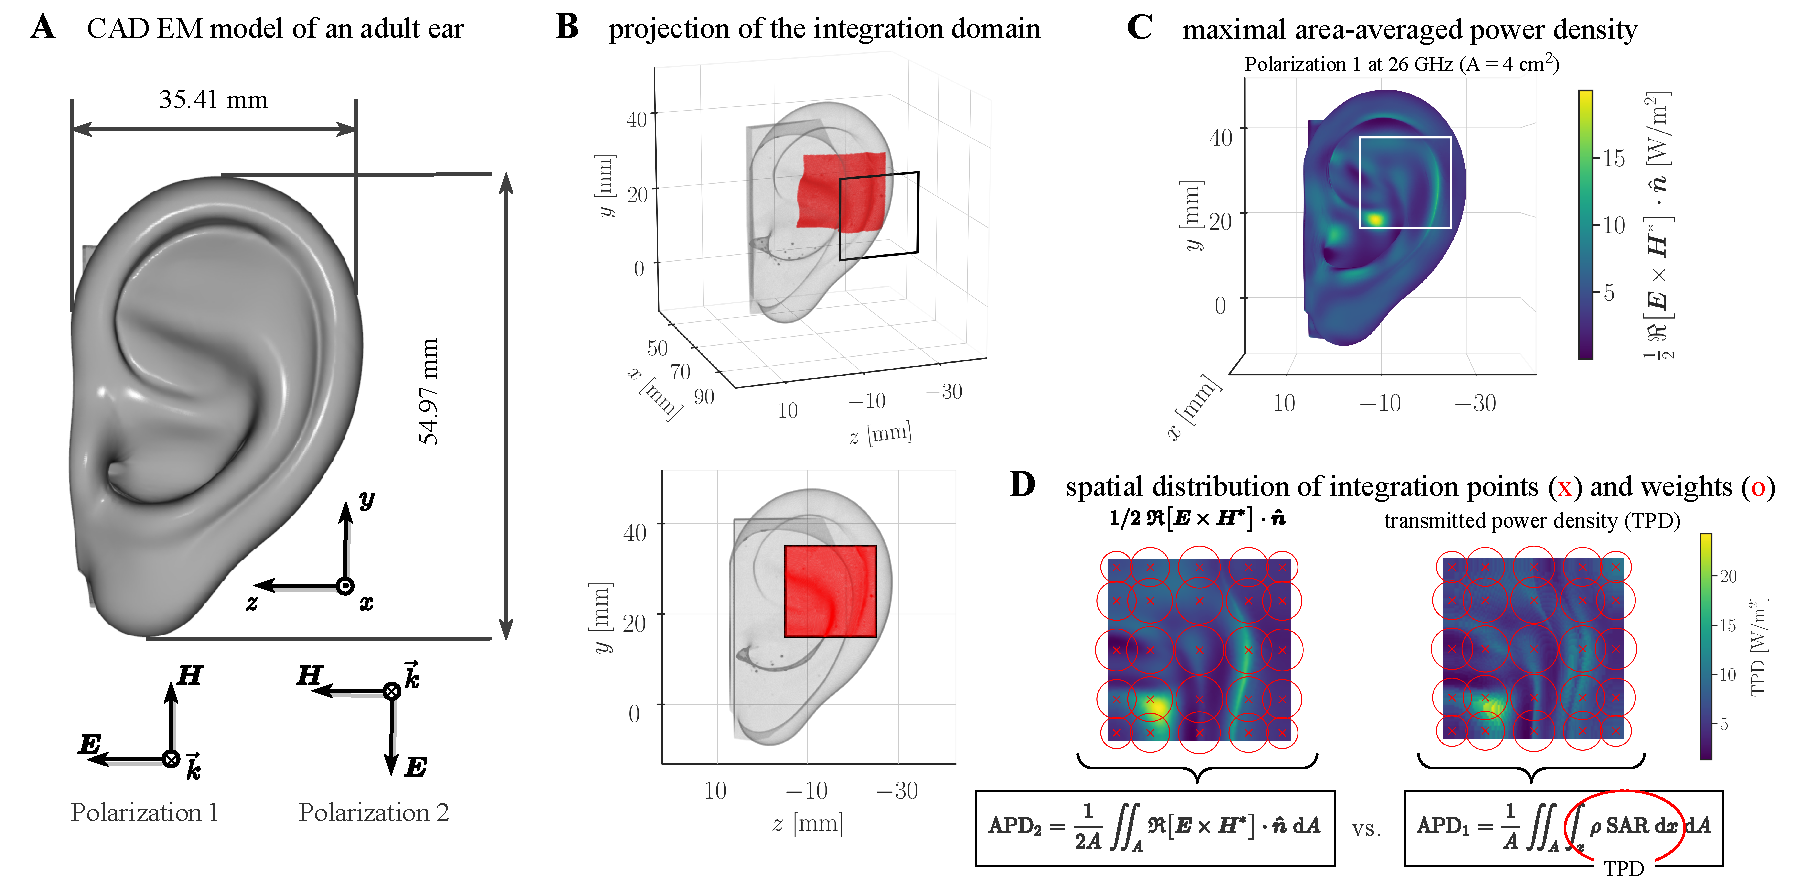
\includegraphics[width=0.95\textwidth]{figures/Kapetanovic2023JERM.pdf}
                \end{figure}
            \end{onlyenv}
            \begin{onlyenv}<9>
                \begin{itemize}
                    \item extension of Kapetanovic, A. Sacco, G., et al. ``Assessment of area-average absorbed power density on realistic tissue models at mmWaves,'' proceedings of \textit{2022 IEEE MTT-S International Microwave Biomedical Conference (IMBioC)}, Suzhou, China -- the best student paper award!
                    \item a new iterative technique for accurate evaluation of the APD on an evaluation surface of arbitrary geometry
                    \item analysis of the plane wave exposure at \SIlist{26;60}{\GHz}
                    \item two definitions of APD compared -- the relative difference within \SI{6}{\percent}
                    \item APD on anatomical model up to \SI{20}{\percent} greater compared to flat tissue models
                \end{itemize}
            \end{onlyenv}
        \end{itemize}
    \end{onlyenv}
\end{frame}

% concluding remarks
\section[Concluding remarks]{Concluding remarks}

\begin{frame}{Main contributions}
    \begin{itemize}
        \item more realistic (non-planar canonical or anatomical) models of human body parts exposed to RF EM fields above 6 GHz, replacing previous flat models
        \item the accurate numerical technique for efficiently evaluating the scalar and vector field surface integrals
        \item the computationally efficient algorithm for automatic detection of ``hot-spots'' regions is developed for proposed models
        \item extensive dosimetric analysis of absorbed and incident EM power density using rigorous mathematical definitions and without simplification of the evaluation surface morphology
    \end{itemize}
\end{frame}

\begin{frame}{Additional contributions}
    \begin{itemize}
        \item confirmation of the validity of APD as BR for maximum superficial temperature rise during local exposure of curved body parts above 6 GHz in steady state
        \item insights into the efficiency of non-planar canonical and anatomical models for EM dosimetry at RF, providing a foundation for future discussions and activities of working group 7 under IEEE/ICES TC 95 SC 6 for EM dosimetry modeling
        \item a basis for discussions on the implementation of non-planar models as reference for future generations of ICNIRP guidelines and IEEE standards
    \end{itemize}
\end{frame}

% standout slide for QnA
\begin{frame}{Questions and answers}
    \centering \LARGE \emph{Thank you!}
\end{frame}

% print all references cited in the document
\begin{frame}[allowframebreaks]{References}
  \printbibliography[heading=none]
\end{frame}

\end{document}
